\documentclass{article}
\usepackage[utf8]{inputenc}
\usepackage{amssymb}
\usepackage{amsmath}
\usepackage{amsfonts}
\usepackage{mathtools}
\usepackage{hyperref}
\usepackage{fancyhdr, lipsum}
\usepackage{ulem}
\usepackage{fontspec}
\usepackage{xeCJK}
\setCJKmainfont[Path = /usr/share/fonts/TTF/]{edukai-5.0.ttf}
\usepackage{physics}
% \setCJKmainfont{AR PL KaitiM Big5}
% \setmainfont{Times New Roman}
\usepackage{multicol}
\usepackage{zhnumber}
% \usepackage[a4paper, total={6in, 8in}]{geometry}
\usepackage[
	a4paper,
	top=2cm, 
	bottom=2cm,
	left=2cm,
	right=2cm,
	includehead, includefoot,
	heightrounded
]{geometry}
% \usepackage{geometry}
\usepackage{graphicx}
\usepackage{xltxtra}
\usepackage{biblatex} % 引用
\usepackage{caption} % 調整caption位置: \captionsetup{width = .x \linewidth}
\usepackage{subcaption}
% Multiple figures in same horizontal placement
% \begin{figure}[H]
%      \centering
%      \begin{subfigure}[H]{0.4\textwidth}
%          \centering
%          \includegraphics[width=\textwidth]{}
%          \caption{subCaption}
%          \label{fig:my_label}
%      \end{subfigure}
%      \hfill
%      \begin{subfigure}[H]{0.4\textwidth}
%          \centering
%          \includegraphics[width=\textwidth]{}
%          \caption{subCaption}
%          \label{fig:my_label}
%      \end{subfigure}
%         \caption{Caption}
%         \label{fig:my_label}
% \end{figure}
\usepackage{wrapfig}
% Figure beside text
% \begin{wrapfigure}{l}{0.25\textwidth}
%     \includegraphics[width=0.9\linewidth]{overleaf-logo} 
%     \caption{Caption1}
%     \label{fig:wrapfig}
% \end{wrapfigure}
\usepackage{float}
%% 
\usepackage{calligra}
\usepackage{hyperref}
\usepackage{url}
\usepackage{gensymb}
% Citing a website:
% @misc{name,
%   title = {title},
%   howpublished = {\url{website}},
%   note = {}
% }
\usepackage{framed}
% \begin{framed}
%     Text in a box
% \end{framed}
%%

\usepackage{array}
\newcolumntype{F}{>{$}c<{$}} % math-mode version of "c" column type
\newcolumntype{M}{>{$}l<{$}} % math-mode version of "l" column type
\newcolumntype{E}{>{$}r<{$}} % math-mode version of "r" column type
\newcommand{\PreserveBackslash}[1]{\let\temp=\\#1\let\\=\temp}
\newcolumntype{C}[1]{>{\PreserveBackslash\centering}p{#1}} % Centered, length-customizable environment
\newcolumntype{R}[1]{>{\PreserveBackslash\raggedleft}p{#1}} % Left-aligned, length-customizable environment   
\newcolumntype{L}[1]{>{\PreserveBackslash\raggedright}p{#1}} % Right-aligned, length-customizable environment
% \begin{center}
% \begin{tabular}{|C{3em}|c|l|}
%     \hline
%     a & b \\
%     \hline
%     c & d \\
%     \hline
% \end{tabular}
% \end{center}  

\usepackage{bm}
% \boldmath{**greek letters**}
\usepackage{tikz}
\usepackage{titlesec}
% standard classes:
% http://tug.ctan.org/macros/latex/contrib/titlesec/titlesec.pdf#subsection.8.2
 % \titleformat{<command>}[<shape>]{<format>}{<label>}{<sep>}{<before-code>}[<after-code>]
% Set title format
% \titleformat{\subsection}{\large\bfseries}{ \arabic{section}.(\alph{subsection})}{1em}{}
\usepackage{amsthm}
\usetikzlibrary{shapes.geometric, arrows}
% https://www.overleaf.com/learn/latex/LaTeX_Graphics_using_TikZ%3A_A_Tutorial_for_Beginners_(Part_3)%E2%80%94Creating_Flowcharts

% \tikzstyle{typename} = [rectangle, rounded corners, minimum width=3cm, minimum height=1cm,text centered, draw=black, fill=red!30]
% \tikzstyle{io} = [trapezium, trapezium left angle=70, trapezium right angle=110, minimum width=3cm, minimum height=1cm, text centered, draw=black, fill=blue!30]
% \tikzstyle{decision} = [diamond, minimum width=3cm, minimum height=1cm, text centered, draw=black, fill=green!30]
% \tikzstyle{arrow} = [thick,->,>=stealth]

% \begin{tikzpicture}[node distance = 2cm]

% \node (name) [type, position] {text};
% \node (in1) [io, below of=start, yshift = -0.5cm] {Input};

% draw (node1) -- (node2)
% \draw (node1) -- \node[adjustpos]{text} (node2);

% \end{tikzpicture}

%%

\DeclareMathAlphabet{\mathcalligra}{T1}{calligra}{m}{n}
\DeclareFontShape{T1}{calligra}{m}{n}{<->s*[2.2]callig15}{}

% Defining a command
% \newcommand{**name**}[**number of parameters**]{**\command{#the parameter number}*}
% Ex: \newcommand{\kv}[1]{\ket{\vec{#1}}}
% Ex: \newcommand{\bl}{\boldsymbol{\lambda}}
\newcommand{\scripty}[1]{\ensuremath{\mathcalligra{#1}}}
% \renewcommand{\figurename}{圖}
\newcommand{\sfa}{\text{  } \forall}
\newcommand{\floor}[1]{\lfloor #1 \rfloor}
\newcommand{\ceil}[1]{\lceil #1 \rceil}


%%
%%
% A very large matrix
% \left(
% \begin{array}{ccccc}
% V(0) & 0 & 0 & \hdots & 0\\
% 0 & V(a) & 0 & \hdots & 0\\
% 0 & 0 & V(2a) & \hdots & 0\\
% \vdots & \vdots & \vdots & \ddots & \vdots\\
% 0 & 0 & 0 & \hdots & V(na)
% \end{array}
% \right)
%%

% amsthm font style 
% https://www.overleaf.com/learn/latex/Theorems_and_proofs#Reference_guide

% 
%\theoremstyle{definition}
%\newtheorem{thy}{Theory}[section]
%\newtheorem{thm}{Theorem}[section]
%\newtheorem{ex}{Example}[section]
%\newtheorem{prob}{Problem}[section]
%\newtheorem{lem}{Lemma}[section]
%\newtheorem{dfn}{Definition}[section]
%\newtheorem{rem}{Remark}[section]
%\newtheorem{cor}{Corollary}[section]
%\newtheorem{prop}{Proposition}[section]
%\newtheorem*{clm}{Claim}
%%\theoremstyle{remark}
%\newtheorem*{sol}{Solution}



\theoremstyle{definition}
\newtheorem{thy}{Theory}
\newtheorem{thm}{Theorem}
\newtheorem{ex}{Example}
\newtheorem{prob}{Problem}
\newtheorem{lem}{Lemma}
\newtheorem{dfn}{Definition}
\newtheorem{rem}{Remark}
\newtheorem{cor}{Corollary}
\newtheorem{prop}{Proposition}
\newtheorem*{clm}{Claim}
%\theoremstyle{remark}
\newtheorem*{sol}{Solution}

% Proofs with first line indent
\newenvironment{proofs}[1][\proofname]{%
  \begin{proof}[#1]$ $\par\nobreak\ignorespaces
}{%
  \end{proof}
}
\newenvironment{sols}[1][]{%
  \begin{sol}[#1]$ $\par\nobreak\ignorespaces
}{%
  \end{sol}
}
%%%%
%Lists
%\begin{itemize}
%  \item ... 
%  \item ... 
%\end{itemize}

%Indexed Lists
%\begin{enumerate}
%  \item ...
%  \item ...

%Customize Index
%\begin{enumerate}
%  \item ... 
%  \item[$\blackbox$]
%\end{enumerate}
%%%%
% \usepackage{mathabx}
\usepackage{xfrac}
%\usepackage{faktor}
%% The command \faktor could not run properly in the pc because of the non-existence of the 
%% command \diagup which sould be properly included in the amsmath package. For some reason 
%% that command just didn't work for this pc 
\newcommand*\quot[2]{{^{\textstyle #1}\big/_{\textstyle #2}}}


\makeatletter
\newcommand{\opnorm}{\@ifstar\@opnorms\@opnorm}
\newcommand{\@opnorms}[1]{%
	\left|\mkern-1.5mu\left|\mkern-1.5mu\left|
	#1
	\right|\mkern-1.5mu\right|\mkern-1.5mu\right|
}
\newcommand{\@opnorm}[2][]{%
	\mathopen{#1|\mkern-1.5mu#1|\mkern-1.5mu#1|}
	#2
	\mathclose{#1|\mkern-1.5mu#1|\mkern-1.5mu#1|}
}
\makeatother



\linespread{1.5}
\pagestyle{fancy}
\title{普通天文學2024作業一}
\author{B11202041 物理二 $ $ 劉晁泓}
% \date{\today}
\date{March 15, 2024}
\begin{document}
\maketitle
\thispagestyle{fancy}
\renewcommand{\footrulewidth}{0.4pt}
\cfoot{\thepage}
\renewcommand{\headrulewidth}{0.4pt}
\fancyhead[L]{普通天文學2024作業一}

Parsec $\sim 3 \times 10^{18} cm$

\begin{enumerate}
	\item[1.] [20分][關於望遠鏡的大小]如果我們使用SDSS的望遠鏡\textbf{直徑2.5公尺},
		觀測某星系曝光1分鐘,
		算出該星系的視星等為22等($m = 22$)之後該測量值的訊噪比(signal/noise ratio)為5,
		在此我們考慮訊噪比(signal to noise ratio)正比於一次曝光所收集到的所有光子數目$N$的$1/2$次方,
		\[
			\frac{S}{N} \propto N_{\text{photon}}^{\frac{1}{2}}
		\]
		請問\\
		\begin{enumerate}
			\item[(a)] 該22星等的星系距離我們約3000Mpc (1Mpc = $10^6$ pc),
				請問他的絕對星等為?

			\item[(a)] 解:\\
				我們先列出一些我們可能會用到的算式:

				\begin{equation}
					m - M = -2.5 \cdot \log_{10} \frac{f_{\text{observed}}}{f_{\text{observed@10pc}}}
				\end{equation}

				\begin{equation}
					m - M = 5 \cdot \log_{10} \frac{d}{\text{pc}} - 5
				\end{equation}

				\begin{equation}
					f_{\text{observed}} = \frac{L}{4 \pi d^2}
				\end{equation}

				\begin{equation}
					f_{\text{observed@10pc}} = \frac{L}{4 \pi (10 \text{pc})^2}
				\end{equation}

				我們整理公式(2)得到:
				\[
					M = m - 5 \cdot \log_{10} \frac{d}{\text{pc}} + 5
				\]
				\[
					\Rightarrow M = 22 - 5 \cdot \log_{10} (3000 \cdot 10^6) + 5
				\]
				\[
					\Rightarrow M = -20.386
				\]

			\item[(b)] 如果我們用GMT望遠鏡\textbf{直徑25.4公尺},
				觀測同一個星系也是曝光1分鐘,
				請問這個觀測的訊噪比會是多少?
				[觀測收集到的光子數正比於望遠鏡的鏡面面積$\times$觀測時間$\times$星系的flux]

			\item[(b)] 解:\\
				由於觀測時間與flux與題幹相比皆為守恆量,
				收集到的光子數比正比於望遠鏡的鏡面面積比,意即:
				\[
					\frac{N_{\text{phot, GMT}}}{N_{\text{phot, SDSS}}} = \frac{25.4^2}{2.5^2}
				\]
				\[
					\Rightarrow \frac{S/N_{\text{GMT}}}{S/N_{\text{SDSS}}} = \sqrt{\frac{N_{\text{phot, GMT}}}{N_{\text{phot, SDSS}}}} = \frac{25.4}{2.5} = 10.16
				\]
				\[
					\Rightarrow \frac{S}{N}_{\text{GMT}} = 10.16 \cdot \frac{S}{N}_{\text{SDSS}} = 50.8
				\]

			\item[(c)] 請問GMT的望遠鏡曝光1分鐘,
				能偵測到訊噪比為5的星系視星等為何?

			\item[(c)] 解:\\
				設此題要求之星系視星等為$m_x$,
				題幹之星系視星等為$m$,
				因偵測到的光子數相同,
				題幹之星系的flux($f$)與此題之星系的flux($f_x$)之比為:
				\[
					\frac{f}{f_x} = \frac{25.4^2}{2.5^2}
				\]
				此題要求之星等可以由此資訊求出:
				\[
					m_x = m - 2.5 \log_{10} \left( \frac{f_x}{f} \right) = 22 - 2.5 \log_{10} \left( \frac{2.5^2}{25.4^2} \right) = 27.034
				\]
				
			\item[(d)] 如果使用GMT觀測22星等的星系,
				之後我們要求訊噪比為5,
				請問所需的曝光時間為何?
				[以上假設用同一個濾鏡。
				這些計算都是實際上天文學家在構思觀測計畫會做的運算]

			\item[(d)] 解:\\
				此小題相較題幹固定的變數為光子數與flux,
				因此曝光時間比會是鏡面面積比的倒數,
				我們如下求得此題要求之曝光時間($t_x$):
				\[
					\frac{t_x}{t} = \frac{2.5^2}{25.4^2}
				\]
				\[
					\Rightarrow t_x = \frac{2.5^2}{25.4^2} \cdot 1 = 9.68 \cdot 10^{-3} (\text{min})
				\]
		\end{enumerate}

		\begin{figure}[H]
			\centering
			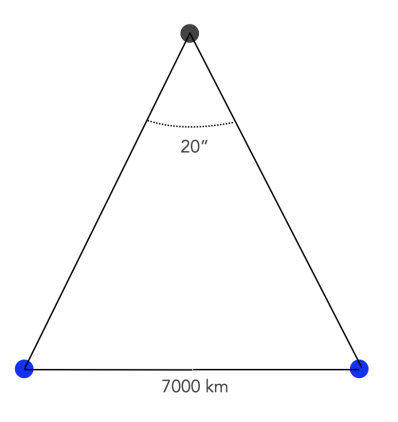
\includegraphics[scale = 0.8]{hw1-1.png}
			\caption{}
			\label{fig1}
		\end{figure}

	\item[2.] [15分][關於視差法] 上課我們提到以前Cassini用視差法量火星距離,
		分別在歐洲和南美洲兩個距離約7000km的地方,量火星的角度變化,
		發現變化角度約為$20''$(20arcsec)(如右圖),
		根據視差法和以上資訊算出地球與火星的距離。

	\item[2.] 解:\\
		設地球火星距離為$x$,
		由於此題角度為角秒的數量級角度甚小,
		我們可以做適當的角度近似:
		\[
			\sin \theta \sim \theta
		\]
		因此我們有
		\[
			x \theta = 3500 (\text{km})
		\]
		\[
			\Rightarrow x = \frac{3500}{10/3600^{\circ}} = 7.219 \cdot 10^7 (\text{km})
		\]

	\item[3.] [15分][關於角解析力] 在2017年,
		天文學家成功使用電波望遠鏡,
		解析了M87超大質量黑定的性質,
		根據廣義相對論,
		該黑洞直徑約$40 \times 10^{12}$公尺,
		而M87離地球約$16 \times 10^6$pc,
		\begin{enumerate}
			\item[(a)] 請估算該黑洞再天空上的角度約?

			\item[(a)] 解:\\
				\[
					\theta = \frac{40 \cdot 10^{12}}{16 \cdot 10^6 \cdot 3 \cdot 10^{16}} (\text{rad}) = \frac{5}{6 \cdot 10^{10}} (\text{rad}) = 1.719 \cdot 10^{-5} ''
				\]

			\item[(b)] 如果在1.3mm的無線電波段觀測,
				要能達到該黑洞再天空上的角度相對應的角解析度,
				請問該望遠鏡的baseline要多長?

				\[
					\theta = 1.22 \frac{\lambda}{D}
				\]
				\[
					\Rightarrow D = 1.22 \frac{\lambda}{\theta} = 1.22 \cdot \frac{1.3 \cdot 10^{-3}}{5/6 \cdot 10^{-10}}(\text{m}) = 1.903 \cdot 10^7 (\text{m})
				\]


			\item[(c)] 請問該baseline的長度,
				跟地球大小相比如何?

			\item[(c)] 地球直徑大小為$12742$公里,
				也就是$1.274 \cdot 10^7$公尺。
				此題算出的望遠鏡直徑約為地球大小的1.5倍,即與地球差不多大。
		\end{enumerate}

	\item[4.] [20分][關於 Period-Luminosity relationship] 我們上課討論到,
		Leavitt 觀測造父變星發現週期和亮度的關係,
		\begin{enumerate}
			\item[(a)] 根據Leavitt實際觀測的數據下圖(x-axis是$\log_{10} P$,y-axis是observed magnitude),
				推算$\alpha$值。

			\item[(a)] 解:\\
				複習一下式(2),
				對於每顆造父變星(我們以$i$作為每顆星的index),
				我們都有:
				\[
					m_{i} - M_{i} = 5 \cdot \log_{10} \left(\frac{d_{i}}{\text{pc}} \right) - 5
				\]
				但是理Leavitt觀測的造父變星們距離銀河系非常遠,
				我們考慮全部造父變星與我們距離近乎相等的近似,
				\[
					d_{i} \sim d \sfa i
				\]
				因此上面的關係式右手邊變成一個與$i$無關的常數:
				\[
					\gamma := 5 \cdot \log_{10} \left(\frac{d}{\text{pc}} \right) - 5
				\]
				現在我們考慮Leavitt的觀測數據,應有:
				\[
					M_i = \alpha \cdot \log_{10} P_i + \beta
				\]
				\[
					\Rightarrow m_i = \alpha \cdot \log_{10} P_i + (\beta + \gamma)
				\]
				利用Leavitt作出的回歸直線(考慮上面那條線大約通過(1.0, 13.5)和(2.0, 11.5)),
				我們有
				\[
					\alpha = \frac{\Delta m}{\Delta \log_{10}P} \sim \frac{11.5 - 13.5}{2.0 - 1.0} = -2
				\]

			\item[(b)] Hertzsrpung 接著觀測銀河系中的造父變星,
				發現週期為6天視星等為4.2mag(這裡我們考慮再上面的那條線,即最亮時的視星等)的造父變星,
				距離為約200pc,
				請用以上資訊推算出$\beta$值。

			\item[(b)] 解:\\
				套用(a)小題推導過的式子,
				我們考慮代入此題提供的數值:
				\[
					m = \alpha \log_{10} P + \beta + 5 \cdot \log_{10} \left( \frac{d}{\text{pc}} \right) - 5
				\]
				\[
					\Rightarrow \beta = m - \alpha \log_{10} P - 5 \cdot \log_{10} \left( \frac{d}{\text{pc}} \right) + 5 
				\]
				\[
					\sim 4.2 - (-2) \cdot \log_{10} 6 + 5 \cdot \log_{10} 200 + 5 = 22.261
				\]

			\item[(c)] 哈伯觀測M31的變星發現週期為30天的變星,
				推算出M31和地球的距離為約900,000光年,
				根據(a)(b)所推算出的週期與光度關係,
				請問該變星的視星等和絕對星等為何?
				[以上有些數值為作業設計,
				並不一定為當時觀測數值]

				\[
					M = \alpha \cdot \log_{10} P + \beta
				\]

			\item[(c)] 解:\\
				絕對星等:
				\[
					M = \alpha \cdot \log_{10} P + \beta = (-2) \cdot \log_{10} 30 + 22.261 = 19.307
				\]
				視星等(1ly $\sim$ 0.3066 pc) :
				\[
					m = M + 5 \cdot \log_{10} \left( \frac{d}{\text{pc}} \right) - 5 = 19.307 + 5 \cdot \log_{10} \left(9 \cdot 10^5 \cdot 0.3066 \right) - 5 = 41.511
				\]
		\end{enumerate}

		\begin{figure}[H]
			\centering
			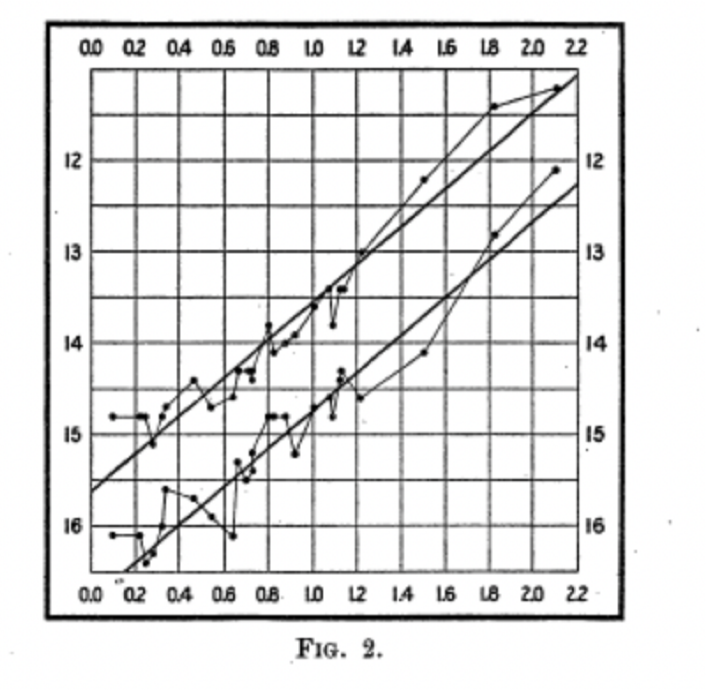
\includegraphics[scale = 0.5]{hw1-2.png}
			\caption{}
			\label{fig2}
		\end{figure}

	\item[5.] [20分][關於望遠鏡] James Webb Space Telescope(JWST)於2021年12/25升空,
		關於它的重要性請讀以下文章
		\href{https://buzzorange.com/citiorange/2022/01/04/hubble-space-telescope/?fbclid=IwAR1CXmTrI6GdBvGQZmgvXEboF2nSSvBRSuHG6GNNWsecLsd9VfA4O6Mj1z}{文章1}
		並請看
		\href{https://www.youtube.com/watch?v=uUAvXYW5bmI&t=231s&ab_channel=JamesWebbSpaceTelescope\%28JWST\%29}{影片1}

		之後回答以下問題:
		\begin{enumerate}
			\item[(a)] JWST約花了多久的時間蓋?

			\item[(a)] 解:\\
				約20年。

			\item[(b)] JWST會飛到哪裡去?

			\item[(b)] 解:\\
				距地球約150萬公里的L2點(拉格朗日點)上。

			\item[(c)] 為什麼JWST需要5層的大帆?

			\item[(c)] 解:\\
				用以阻擋太陽、地球、月球散發出的熱量,
				以提昇偵測來自宇宙的紅外光的準確度。

			\item[(d)] 為什麼JWST需要冷卻到很低溫,
				跟我們上課的哪個物理效應有相關?

			\item[(d)] 解:\\
				因為JWST本身的熱輻射也會影響到他的測量數據,
				此即上課提到的黑體輻射的效應。

			\item[(e)] 根據那個物理效應,JWST的觀測波長範圍($\sim$10 micron)所對應的溫度大約為何?

			\item[(e)] 解:\\
				根據Wien's Law,
				我們有:
				\[
					\lambda T = 0.29 \text{cm} \cdot \text{K}
				\]
				\[
					\Rightarrow T = \frac{0.29}{10 \cdot 10^{-4}} = 290 \text{K}
				\]
		\end{enumerate}

	\item[6.] [10分] 請根據下圖中的四個恆星光譜,
		估算這四個恆星的表面溫度約為多少K?
		請寫出估算方式以及最後算出的恆星1 2 3 4的溫度。
		(資料來源SDSS)
		\begin{figure}
			\centering
			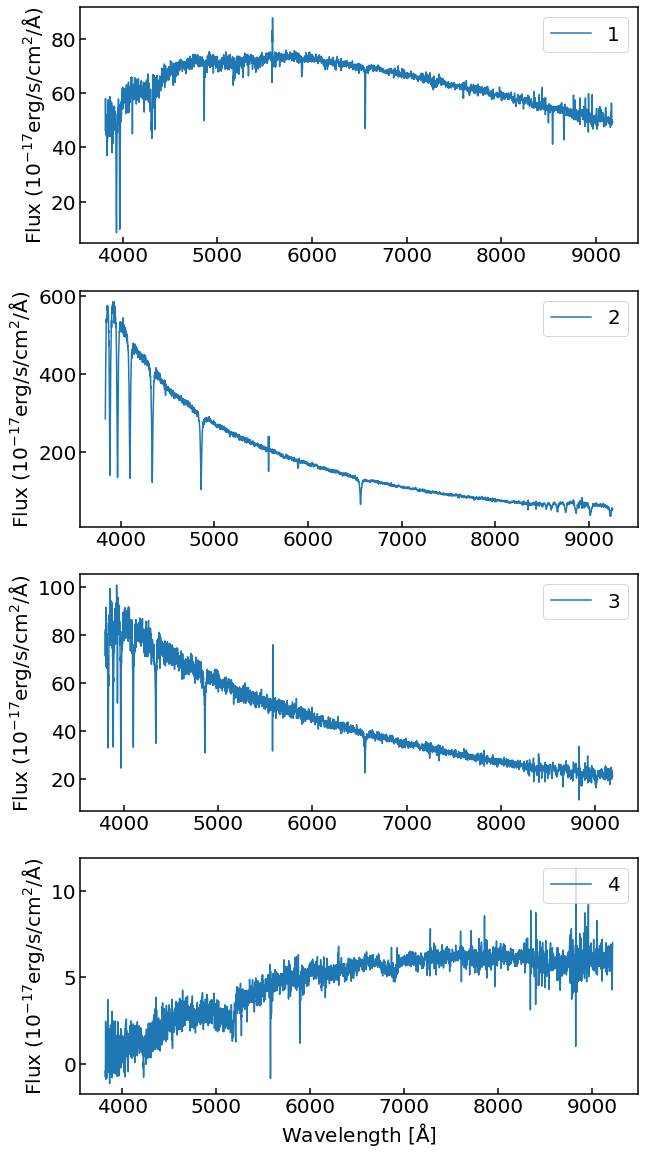
\includegraphics[scale = 0.5]{hw1-3.png}
			\caption{}
			\label{fig3}
		\end{figure}

	\item[6.] 解:\\
		我們應用wien's law,
		先估計$\lambda$的峰值再計算溫度。
		\begin{enumerate}
			\item[(1)] $\lambda \sim 5500 \text{\r{A}}$
				\[
					\Rightarrow T = \frac{0.29}{5500 \cdot 10^{-8}} \sim 5273 \text{K}
				\]

			\item[(2)] $\lambda \sim 4000 \text{\r{A}}$
				\[
					\Rightarrow T = \frac{0.29}{4000 \cdot 10^{-8}} \sim 7250 \text{K}
				\]
				
			\item[(3)] $\lambda \sim 4000 \text{\r{A}}$
				\[
					\Rightarrow T = \frac{0.29}{4000 \cdot 10^{-8}} \sim 7250 \text{K}
				\]

			\item[(4)] $\lambda \sim 8500 \text{\r{A}}$
				\[
					\Rightarrow T = \frac{0.29}{8500 \cdot 10^{-8}} \sim 3411 \text{K}
				\]
		\end{enumerate}


\end{enumerate}




















\end{document}



